\documentclass[border=4pt]{standalone}
\usepackage{tikz}
\usetikzlibrary{arrows,positioning}
\begin{document}
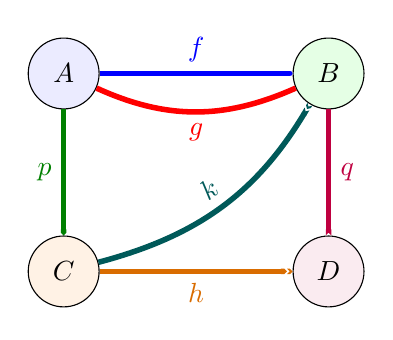
\begin{tikzpicture}[
  node distance=1.6cm and 2.45cm,
  obj/.style={draw,circle,minimum size=9mm,inner sep=1pt}
]
  \node[obj,fill=blue!8] (A) {$A$};
  \node[obj,fill=green!10,right=of A] (B) {$B$};
  \node[obj,fill=orange!10,below=of A] (C) {$C$};
  \node[obj,fill=purple!8,right=of C] (D) {$D$};

  \draw[blue,line width=2pt,-{round cap}] (A) -- node[above] {$f$} (B);
  \draw[red,line width=2pt,-{butt cap}] (B) to[bend left=24] node[below] {$g$} (A);
  \draw[green!50!black,line width=2pt,-{triangle 90 cap}] (A) -- node[left] {$p$} (C);
  \draw[purple,line width=2pt,-{triangle 90 cap reversed}] (B) -- node[right] {$q$} (D);
  \draw[orange!85!black,line width=2pt,-{fast cap}] (C) -- node[below] {$h$} (D);
  \draw[teal!70!black,line width=2pt,-{fast cap reversed}] (C) to[bend right=22] node[above,sloped] {$k$} (B);
\end{tikzpicture}
\end{document}
